%%%% SEITENRAENDER, SCHRIFTGROESSE UND ZEILENABSTAND NICHT ABAENDERN => SONST GIBT ES PUNKTEABZUG
\documentclass[a4paper,11pt,singlespacing]{article}
% \usepackage[left=2.5cm,right=2.5cm,top=2.5cm]{geometry}
\usepackage{setspace}
\usepackage[utf8]{inputenc}
\usepackage[T1]{fontenc}
\usepackage{graphicx}
\usepackage[ngerman]{babel}
\usepackage{color}
\usepackage{wrapfig}
\usepackage{titleref}
\usepackage{hyperref}
\usepackage[rightcaption]{sidecap}
\usepackage{listings,xcolor}
\usepackage[numbers,round]{natbib}

% Configuration
\sloppy
\setlength{\parindent}{0ex} % Absatzeinrückung verhindern
\graphicspath{ {images/} }

\begin{document}
\pagenumbering{roman}

% Cover
\title{Systemadministration - Mailserver Honypot zum analysieren von Spam}
\author{Manuel Adams 27470, Michael Ruf 27428, Mario Waizenegger 29608}
\maketitle
\begin{abstract}
Heutzutage wird viel Spam verschickt. Einiges davon wird erkannt und gefiltert.
Das Projekt befasst sich zum einen mit der Aufgabe Spam zu erhalten und zum anderen als Verteiler für den Versandt von Spammails zu dienen.
Damit soll das Verhalten der Spammer und die konkreten Spam Nachrichten analysiert werden.
\\\\
Zur Durchführung wird hierzu ein Spam Honeypot aufgesetzt.
Um die nötigen Daten zu erhalten wird der Mail-Server offen publiziert und durch mehreren Mail-Adressen bei ominösen Diensten registriert.
\\\\
Das Ziel des Projektes ist ...\color{red}{TODO}
\end{abstract}

\newpage

% Table of contents
\tableofcontents

\newpage
\pagenumbering{arabic}

% Content
\section{Einleitung/Motivation}\label{sec:Einleitung}

	\subsection{Ziel der Arbeit}\label{sec:Ziel}
		Es sollen durch einen Mailserver Honeypot Erkenntnisse über Herkunft, Zweck und Zielgruppe von Spam Nachrichten erhalten werden.
		Durch diese Informationen soll die die Motivation von Spammern besser verstanden und entsprechende Vorkehrungen zum Schutz erzielt werden können.
		% TODO Bisschen kurz

	\subsection{Motivation}\label{sec:Motivation}
		Die Nachvollziehbarkeit für das Versenden vom Spam ist vielen Menschen ein Rätsel.
		Dies wirft die Fragen auf wieso jemand Spam verschicken sollte, wer Spam verschickt und warum.
		Was passiert wenn man auf Spam absichtlich reagiert?
		Ein Spam Honeypot bietet die Möglichkeit diese Fragen zu analysieren und die Daten zu erheben.
		Die Einrichtung, das Publizieren unter Spammern und der Erhalt vieler Spam Mails in kurzer Zeit ist eine gute Herausforderung.
		% - Wirtschaftlichkeit
		% - Andere Beweggründe
		% - Findet man Informationen über Systeme, von denen Spam verschickt wird?
		% - Werden die Nachrichten generiert? (Bots)
	
	\subsection{Vorgehensweise}\label{sec:Vorgehensweise}
		Eingangsserver
		\begin{enumerate}
		\item Mail Eingangsserver bereitstellen und konfigurieren
		\item DNS Server einrichten um realistische E-Mail-Adressen bereitzustellen
		\item Bei möglichst vielen Diensten mit unterschiedlichen Mailadressen registrieren
		\item Mails analysieren
		\end{enumerate}

		Ausgangsserver ("Open Relay") % TODO Ref
		\begin{enumerate}
		\item Mail Ausgangsserver bereitstellen und konfigurieren
		\item Als "Open Relay" im Internet durchsickern lassen % TODO Ref
		\item Eingehende Mails tatsächlich weiterleiten
		\item Mails analysieren
		\end{enumerate}

	\subsection{Aufbau der Arbeit}\label{sec:Aufbau}
		Die Hochschule Weingarten stellt für das Projekt eine Virtuelle Maschine (VM) zur Verfügung. %TODO Ref VM
		Auf dieser werden die Dienste in (virtualisierten) Containern aufgesetzt. % TODO Ref Container
		Die VM muss aus Sicherheitsgründen ins interne Netz abgeschottet sein.
		Nach Außen soll der Mail-Dienst zur Nutzung als Honeypot verfügbar sein.

		Das Bild \ref{fig:structure} beschreibt den Aufbau.

		\begin{figure}
		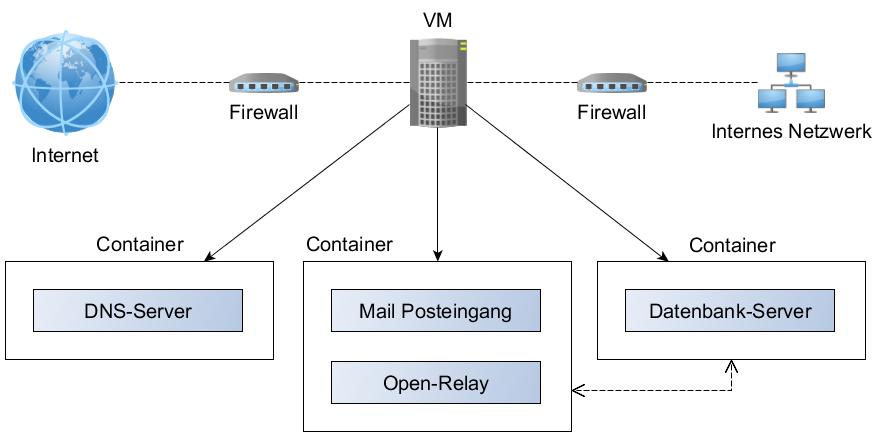
\includegraphics[width=\linewidth]{2-Hierarchy.png}
		\caption{Projektstruktur}
		\label{fig:structure}
		\end{figure}


\section{Grundbegriffe}\label{sec:Grundbegriffe}
	Die folgenden Begriffsdefinitionen und Unterscheidungen sind zum einen zur Verdeutlichung, wie Begriffe in dieser Arbeit verstanden werden und um Fachbegriffe zu erklären.
	
	\begin{description}
	% TODO Honeypot
	\item[Open relay\label{itm:OpenRelay}]\hfill \\
		Ein SMTP-Relay-Server der durch unzureichende Sicherheitskonfiguration auch Mails weiterleitet bei denen er weder für die Absender- noch für die Zieladresse zuständig ist, wird als "`Open relay"' bezeichnet.\cite{SMTP-Relay-Server}
	% TODO VM
	% TODO Container
	\end{description}


\section{Problemstellung}\label{sec:Problemstellung}
	% Mario
	In der heutigen Zeit ist jeder mit dem Thema Spam konfrontiert und damit wie ein guter Schutz gegen Spammails realisiert werden kann.	
	
	Um die Ziele von Spammern besser verstehen zu können, aber auch deren Zielgruppen zu ermitteln, sollen durch einen Mailserver Honypot Spamnachrichten empfangen/weitergeleitet und analysiert werden. 
	Dabei soll der Mailserver durch unzureichende Sicherheitskonfiguration (\nameref{itm:OpenRelay}) für potentielle Spammer interessant gemacht werden und damit als Ausgangsserver für den Versand von Spam Mails dienen.
	
	Außerdem sollen unauffällige Mailadressen durch Anmeldung an ominösen Diensten und Plattformen im Netz verteilt werden, sodass an diese Adressen Spam empfangen werden kann.
\\
	Die Schwierigkeiten bei der Umsetzung für das \nameref{itm:OpenRelay} sind, dass der Server in der Spam-Community bekannt und akzeptiert werden muss, aber dieser auch möglichst lange nicht auf den "`\nameref{itm:OpenRelay}"'"~Blacklists auftaucht.
	
	Bei der Verteilung von Mailadressen, könnten diese möglicherweise im Projektzeitraum nicht ausreichend verbreitet werden und somit nur wenige Spammails empfangen werden.
\\\\
	% Manu
	Um bei Spammern als offener Relay-Server bekannt zu werden könnte es Monate dauern, daher muss noch eine Möglichkeit gefunden werden, diesen Prozess zu beschleunigen.
	Um den Empfang von Spam zu beschleunigen werden von uns verschiedene E-Mail-Adressen bei Socialmedia-Seiten und anderen unsicheren Seiten registriert.
	Im Fall von Spam Empfang sollen dann auch eventuelle Links und Bilder in den Nachrichten geöffnet werden um die Aktivität der Mail für den Spammer anzuzeigen.


\section{Anforderungsanalyse/Priorisierung}\label{sec:AnforderungsanalysePriorisierung}
	\begin{itemize}
	\item Der Mail-Server muss unter Spammern publik gemacht werden.
	\item Der Mail-Server muss über DNS Einträge Mails signieren und weiter versenden können.
	\item Der Mail-Server muss als Mail-Relay-Server aufgesetzt werden.
	\item Es muss sichergestellt werden das Dritte keinen unberechtigten Zugriff auf die VM erhalten.
	\end{itemize}


\section{Lösungsvorschläge}\label{sec:Lösungsvorschläge}
	TODO


\section{Auswahl Lösung anhand Anforderungen}\label{sec:AuswahlLösungAnhandAnforderungen}
	TODO


\section{Umsetzung}\label{sec:Umsetzung}
	TODO


\section{Fazit/Ausblick/Übertragbarkeit}\label{sec:Fazit/Ausblick/Übertragbarkeit}
	TODO


\newpage

% Quotes
\bibliography{zitate}
\bibliographystyle{plain}
\addcontentsline{toc}{section}{Literatur}

% Image listing
\listoffigures
\addcontentsline{toc}{section}{Abbildungsverzeichnis}

% TODO What are listings?! -> Code examples
\lstlistoflistings
\addcontentsline{toc}{section}{Listings}

\newpage

% Additional stuff
\section*{Anhang}\label{Anhang}
\addcontentsline{toc}{section}{Anhang}

\newpage

% Plagiarism declaration
\section*{Eidesstattliche Erklärung}\label{sec:Eidesstattliche Erklärung}


\end{document}